\documentclass[10pt,a4paper]{article}
\usepackage[latin1]{inputenc}
\usepackage{amsmath}
\usepackage{amsfonts}
\usepackage{amssymb}
\usepackage{graphicx}
\usepackage{multicol}
\usepackage{changepage}
\usepackage{float}
\usepackage{cite}
\usepackage{url}
\usepackage{imakeidx}
\makeindex

\usepackage[left=2.50cm, right=2.50cm]{geometry}
\usepackage[spanish]{babel}

\author{Axel}
\title{Portada siempre practica}

\begin{document}
%encabezado 
\pagestyle{plain}{
\pagestyle{empty}
\changepage{3cm}{1cm}{-0.5cm}{-0.5cm}{}{-2cm}{}{}{}
\noindent

%sEGIUN EL formato de sus imagenes, deben encontrar una configuracion adeacuada para ustedes
{\small
\begin{tabular}{p{0.626\textwidth} p{0.50\textwidth} }

\includegraphics[scale=0.26]{uaem.jpg} &  
\includegraphics[scale=0.3]{ico.jpg}
\end{tabular}
}

%datos de la caratula
\begin{center}
\par\vspace{2cm} %espacio dejado antes del encabezado
{
\Huge\textbf{
Universidad Aut\'onoma del Estado de M\'exico \\[1cm] Ingenier\'ia en Computaci\'on
}
}
\par\vspace{1.5cm}
{
\Large\textbf{ Materia: Algoritmos Gen\'eticos \\ Proyecto 2
}
}
\par\vspace{1.5cm}
{
\large\textbf{Axel Valenzuela Ju\'arez \\Profesor: Dr. Asdr\'ubal	L\'opez	Chau \\ 31 de Marzo del 2020 } 
}

\par\vspace{1.5cm}

\end{center}
\clearpage

}

\printindex

\section{
Introducci\'on
}

\paragraph{
Los Algoritmos Gen\'eticos son m\'etodos adaptativos que pueden usarse para resolver problemas de b\'usqueda y optimizaci\'on. Est\'an basados en el proceso gen\'etico de los organismos vivos.
}
\paragraph{
Los Algoritmos Gen\'eticos son capaces de ir creando soluciones para problemas del mundo real.
}
\paragraph{
El poder de los Algoritmos Gen\'eticos proviene del hecho de que se trata de una t\'ecnica robusta,
y pueden tratar con \'exito una gran variedad de problemas provenientes de diferentes \'areas, incluyendo aquellos en los que otros m\'etodos encuentran dificultades. Si bien no se garantiza que el Algoritmo Gen\'etico encuentre la soluci\'on optima del problema, existe evidencia emp\'irica de que se encuentran soluciones de un nivel aceptable, en un tiempo competitivo con el resto de los algoritmos de optimizaci\'on combinatoria. En el caso de que existan t\'ecnicas especializadas para resolver un determinado problema, lo m\'as probable es que superen al Algoritmo Gen\'etico, tanto en rapidez como en eficacia.
}
\paragraph{
 El gran campo de aplicaci\'on de los Algoritmos Gen\'eticos se relaciona con aquellos problemas para los cuales no existen t\'ecnicas especializadas. Incluso en el caso en que dichas t\'ecnicas existan, y funcionen bien, pueden efectuarse mejoras de estas hibrid\'andolas con los Algoritmos Gen\'eticos.
}
\newpage
\section{Desarrollo}


\paragraph{El problema de las cartas consiste en un conjunto de cartas del 2 al 10 y el as que se separan en dos grupos de 5 cartas, las cartas de cada grupo tendrá diferentes restricciones.}

\paragraph{En el primer grupo las cartas deben tener un producto de 360 y en el otro grupo los valores deben sumar 36. Solo se pueden usar una vez las cartas.}

\paragraph{
La primer parte del algoritmo funciona correctamente pero el algoritmo se traba ya que el algoritmo tiene que cambiar dos n\'umeros, eso es lo que a continuaci\'on se busca hacer.
}

\begin{figure}[H]
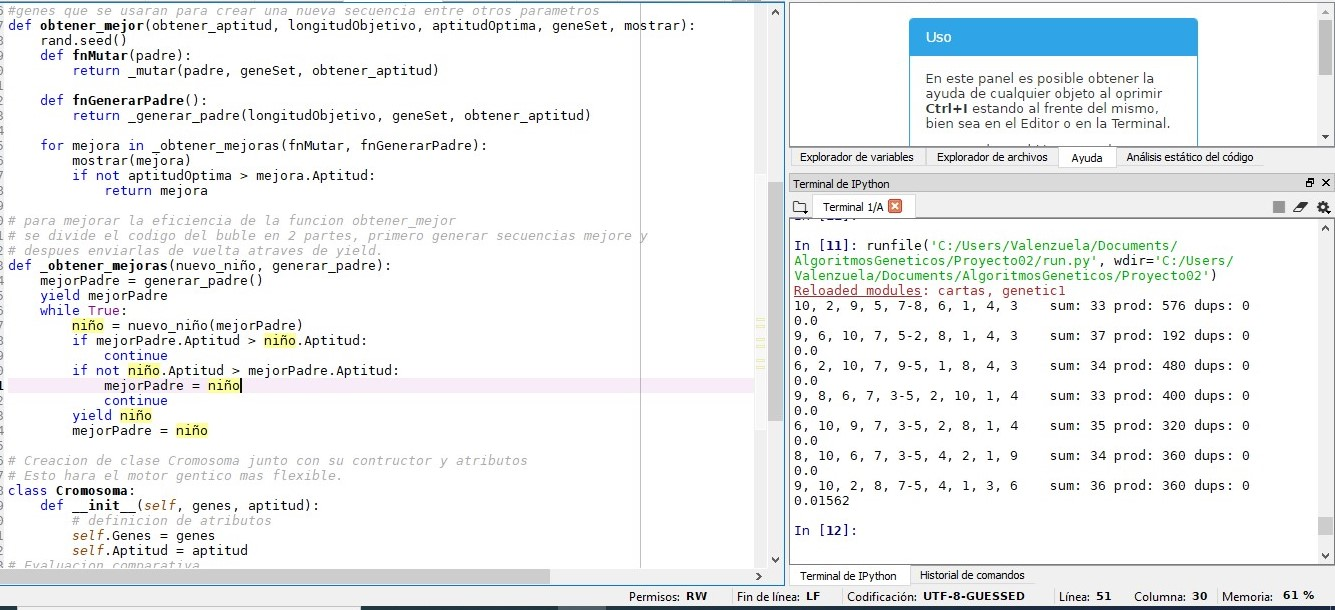
\includegraphics[scale=0.4] {CambiosGenetic.jpg}
\caption{Cambios en el archivo genetic.}
\label{fig:cod1}
\end{figure}



\paragraph{
En la segunda prueba del algoritmo se hicieron los cambios posibles para cambiar los dos n\'umeros, para esto fue necesario mover a el archivo genetic.py, aun as\'i despu\'es de ejecutar este segundo intento se volvieron a tener problemas con la ejecuci\'on. Para resolver esto fue necesario mejorar la funci\'on mutar del archivo cartas.py. Ref:\ref{fig:cod2}
}


\begin{figure}[H]
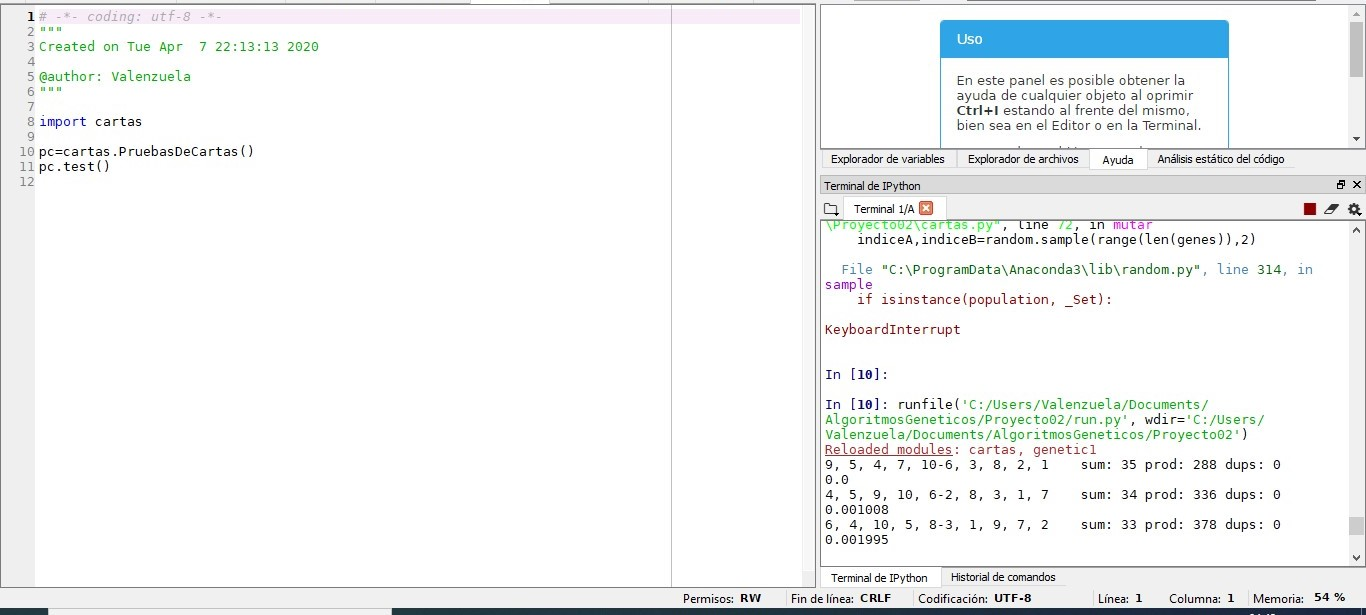
\includegraphics[scale=0.4] {segundaprueba.jpg}
\caption{Resultados de la segunda prueba.}
\label{fig:cod2}
\end{figure}


\paragraph{Una vez que se mejor\'o la funci\'on y se volvi\'o a ejecutar se puedo observar que el error fue arreglado y esta vez el algoritmo fue correctamente terminado. Ref: \ref{fig:cod3}
}

\begin{figure}[H]
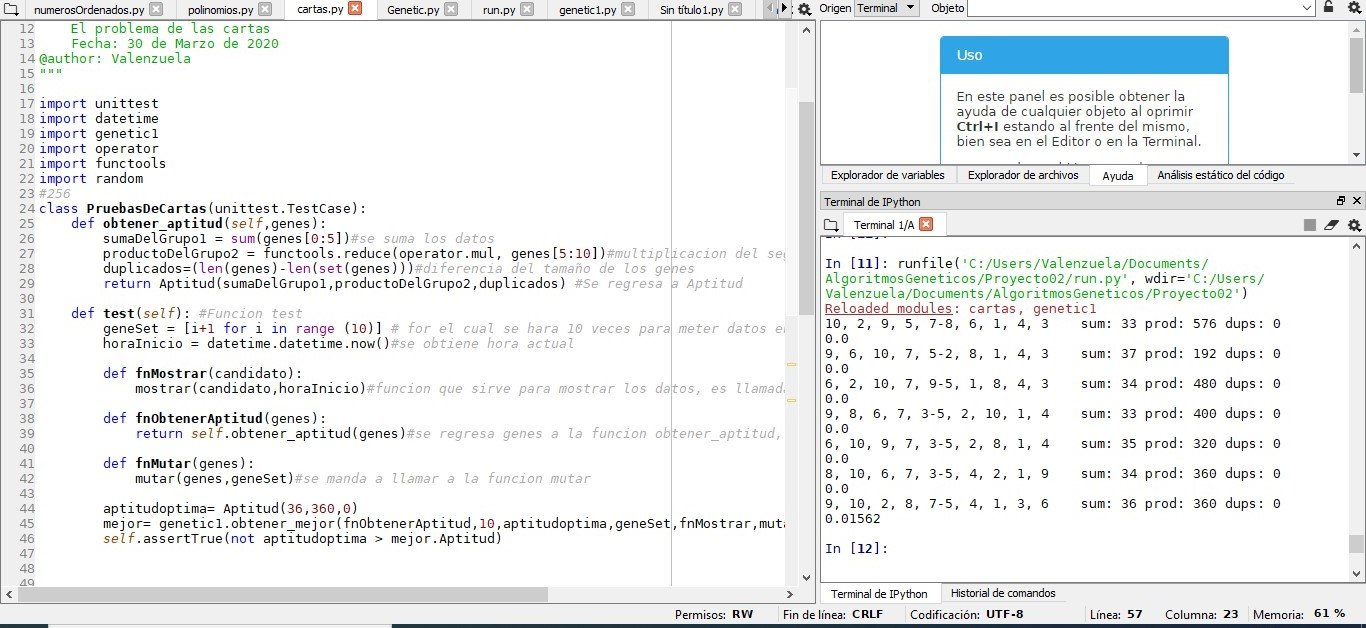
\includegraphics[scale=0.4] {TercerPrueba.jpg}
\caption{Resultados de la tercer prueba.}
\label{fig:cod3}
\end{figure}




\section{Conclusi\'on}
\paragraph{El problema de las cartas es un problema que me costa bastante entender, asi que tuve que investigar mas al respecto y repasar el recurso que nos proporciono para entender.}
\paragraph{
Esta pr\'actica nos hace aprender aun mas los casos pr\'acticos que tienen los algoritmos gen\'eticos, aumentamos un poco mas la complejidad de el archivo genetic para resolver este problema en espec\'ifico y gracias a el fragmento del libro se logr\'o solucionar el problema de las cartas.}
\paragraph{
Para finalizar creo que seria bueno una retroalimentaci\'on de este problema mas espec\'ificamente, entiendo la mayor parte del c\'odigo pero algunas partes pueden ser dif\'iciles de entender.
}
\section{Referencias}
\paragraph{(2019). Algoritmos Gen\'eticos Con Python}
\end{document}
